\documentclass[10pt, conference, compsocconf]{IEEEtran}
\usepackage{graphicx}
\usepackage{float}
\hyphenation{op-tical net-works semi-conduc-tor}
\begin{document}
\title{Latest Data Report}
\author{\IEEEauthorblockN{Song Li}
\IEEEauthorblockA{Lehigh University\\
sol315@lehigh.edu\\
auto generated in \today}
}
\maketitle
\section{Based On Based on Client ID}
\subsection{Basic Numbers}
\begin{itemize}\item We have 450591 fingerprints in total\item We have 336834 users in total\item We have 249021 fingerprintable users in total (73.93\%)\item We have 182217 users only have one fingerprint \end{itemize}\subsection{How many users changed in days}
\begin{figure}[H]\centering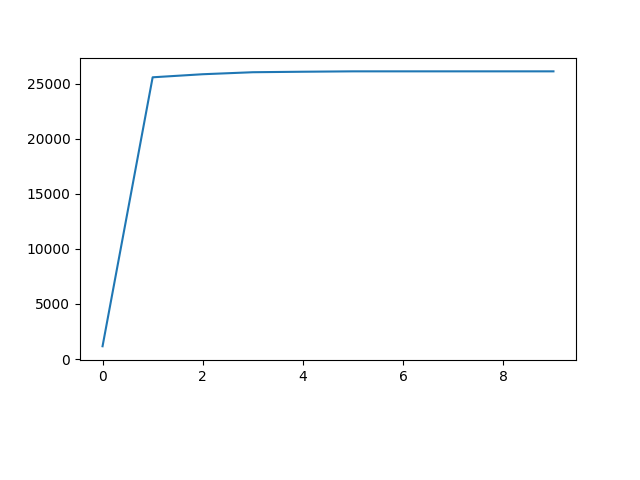
\includegraphics[width=75mm,scale=0.5]{BasedonClientIDchangebytime}\end{figure}\subsection{How many changes for every feature}
\begin{figure}[H]\centering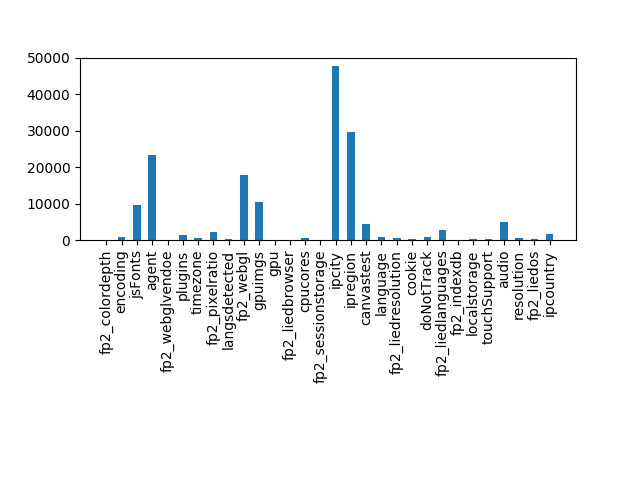
\includegraphics[width=75mm,scale=0.5]{BasedonClientIDfeaturechange}\end{figure}\subsection{How many fingerprints have multiple users}
\begin{figure}[H]\centering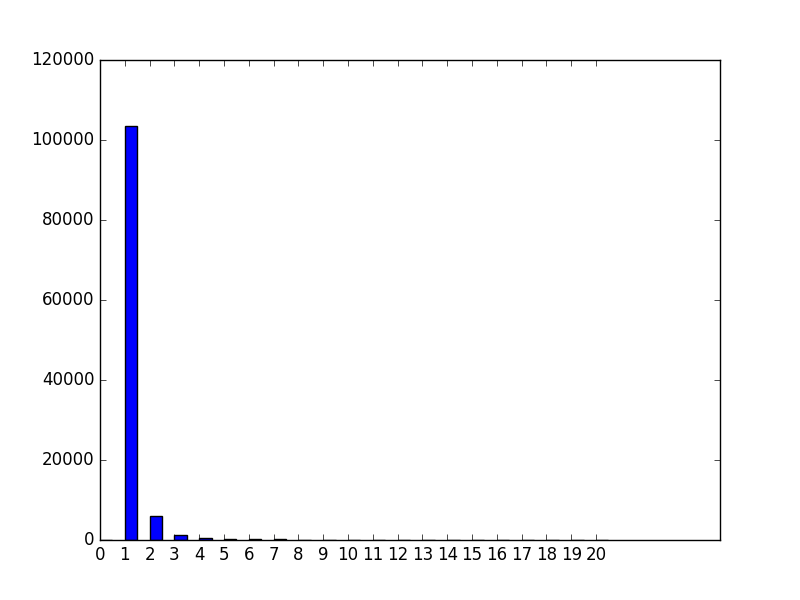
\includegraphics[width=75mm,scale=0.5]{BasedonClientIDnumberofusersfingerprint}\end{figure}\subsection{The percentage of tolerance}
\begin{figure}[H]\centering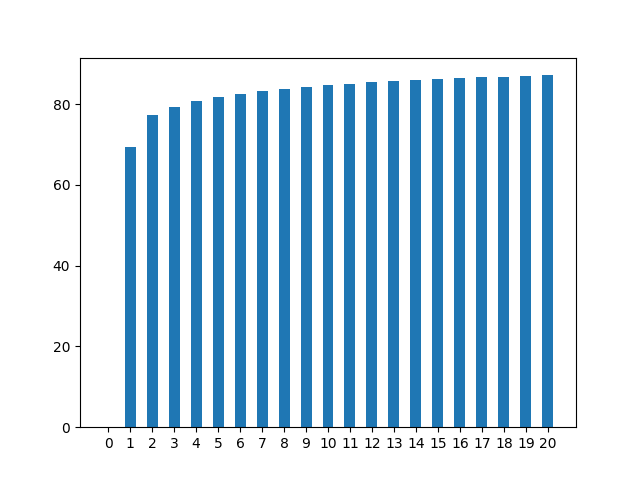
\includegraphics[width=75mm,scale=0.5]{BasedonClientIDtolerance}\end{figure}[0.0, 69.42262360688053, 77.2018264189482, 79.3862852324884, 80.74659921504362, 81.80171835384789, 82.6472386991812, 83.25733150453932, 83.80834476329588, 84.3035441790318, 84.72986693742318, 85.09621950278179, 85.45129054667878, 85.77073573332858, 86.03852342696996, 86.31165499919842, 86.50225333547088, 86.6655385145205, 86.83535510073212, 87.00665609766234, 87.18062903388612]\subsection{location change speed per hour}
\begin{figure}[H]\centering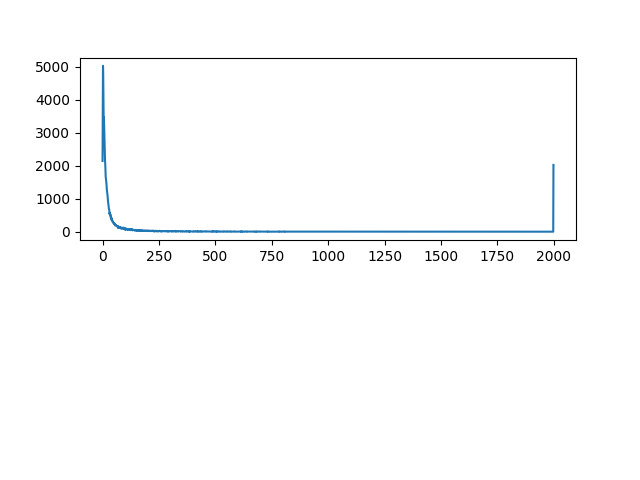
\includegraphics[width=75mm,scale=0.5]{BasedonClientIDlocationchange}\end{figure}\subsection{The distribution of cookie}
\begin{figure}[H]\centering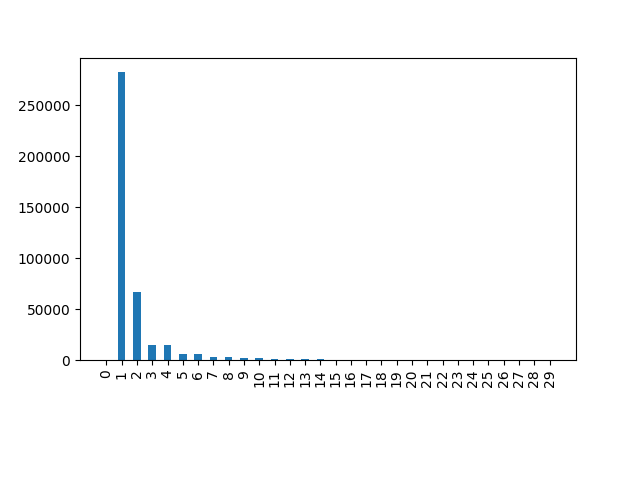
\includegraphics[width=75mm,scale=0.5]{BasedonClientIDcookiedis}\end{figure}[0, 235686, 55294, 11356, 12327, 4618, 4878, 2348, 2388, 1393, 1327, 881, 774, 584, 494, 355, 318, 260, 241, 164, 150, 109, 96, 76, 81, 63, 50, 41, 41, 34]
\end{document}


